% TEXINPUTS=.:$HOME/git/bvtex: latexmk  -pdf <main>.tex
\documentclass[xcolor=dvipsnames]{beamer}

\input{defaults}
\input{beamer/preamble}

\setbeamertemplate{navigation symbols}{}
% \setbeamertemplate{background}[grid][step=1cm]

\usepackage{siunitx}
\usepackage{xmpmulti}
\usepackage[export]{adjustbox}
\usepackage{ulem}
\usepackage[outline]{contour}
\usepackage{pdfpages}
\usepackage{tikz}
\usetikzlibrary{shapes.geometric, arrows}
\usetikzlibrary{positioning}

\definecolor{bvtitlecolor}{rgb}{0.98, 0.92, 0.84}
\definecolor{bvoutline}{rgb}{0.1, 0.1, 0.1}

\renewcommand{\bvtitleauthor}{Brett Viren\\(for WCT team)}
\renewcommand{\bvtit}{WCT}
\renewcommand{\bvtitle}{\LARGE Wire Cell Toolkit\\Updates and Status}
\renewcommand{\bvevent}{SimReco\\2017 May 18}
\renewcommand{\bvbeamerbackground}{}

\def\Put(#1,#2)#3{\leavevmode\makebox(0,0){\put(#1,#2){#3}}}


\begin{document}
\input{beamer/title.tex}
\input{beamer/toc.tex}

\section{Simulation}

\begin{frame}
  \frametitle{WCT Simulation Scope}
  Overview:
  \begin{description}
  \item[Energy depositions] ideal, parameterized line sources or
    detailed deposition from file (LArG4 dumps: \textbf{Brooke})
  \item[Drift physics] Fano factor, recombination, absorption,
    diffusion and related statistics (\textbf{Hanyu})
  \item[Response] long-range/fine-grained DUNE and $\mu$BooNE 2D
    Garfield field (\textbf{Yichen}) and electronics (\textbf{Huchen}) responses.
  \item[Wire geometry] 3D wires from file or parameterized generator.
  \item[Convolution] $Q_{drift} \otimes R_{field} \otimes R_{elec}$
    optimized for RAM and CPU \\
    {\footnotesize (200 MB max RAM, 20k depos/minute)}.
  \item[Noise] empirical $\mu$BooNE (\textbf{Jyoti}) and first principle 
    (\textbf{Milind/Arbin}) noise models, in development.
  \item[Digitizer] simple, parameterized linear model.
  \end{description}
\end{frame}

\begin{frame}
  \frametitle{DUNE Field Responses}
  \begin{center}
    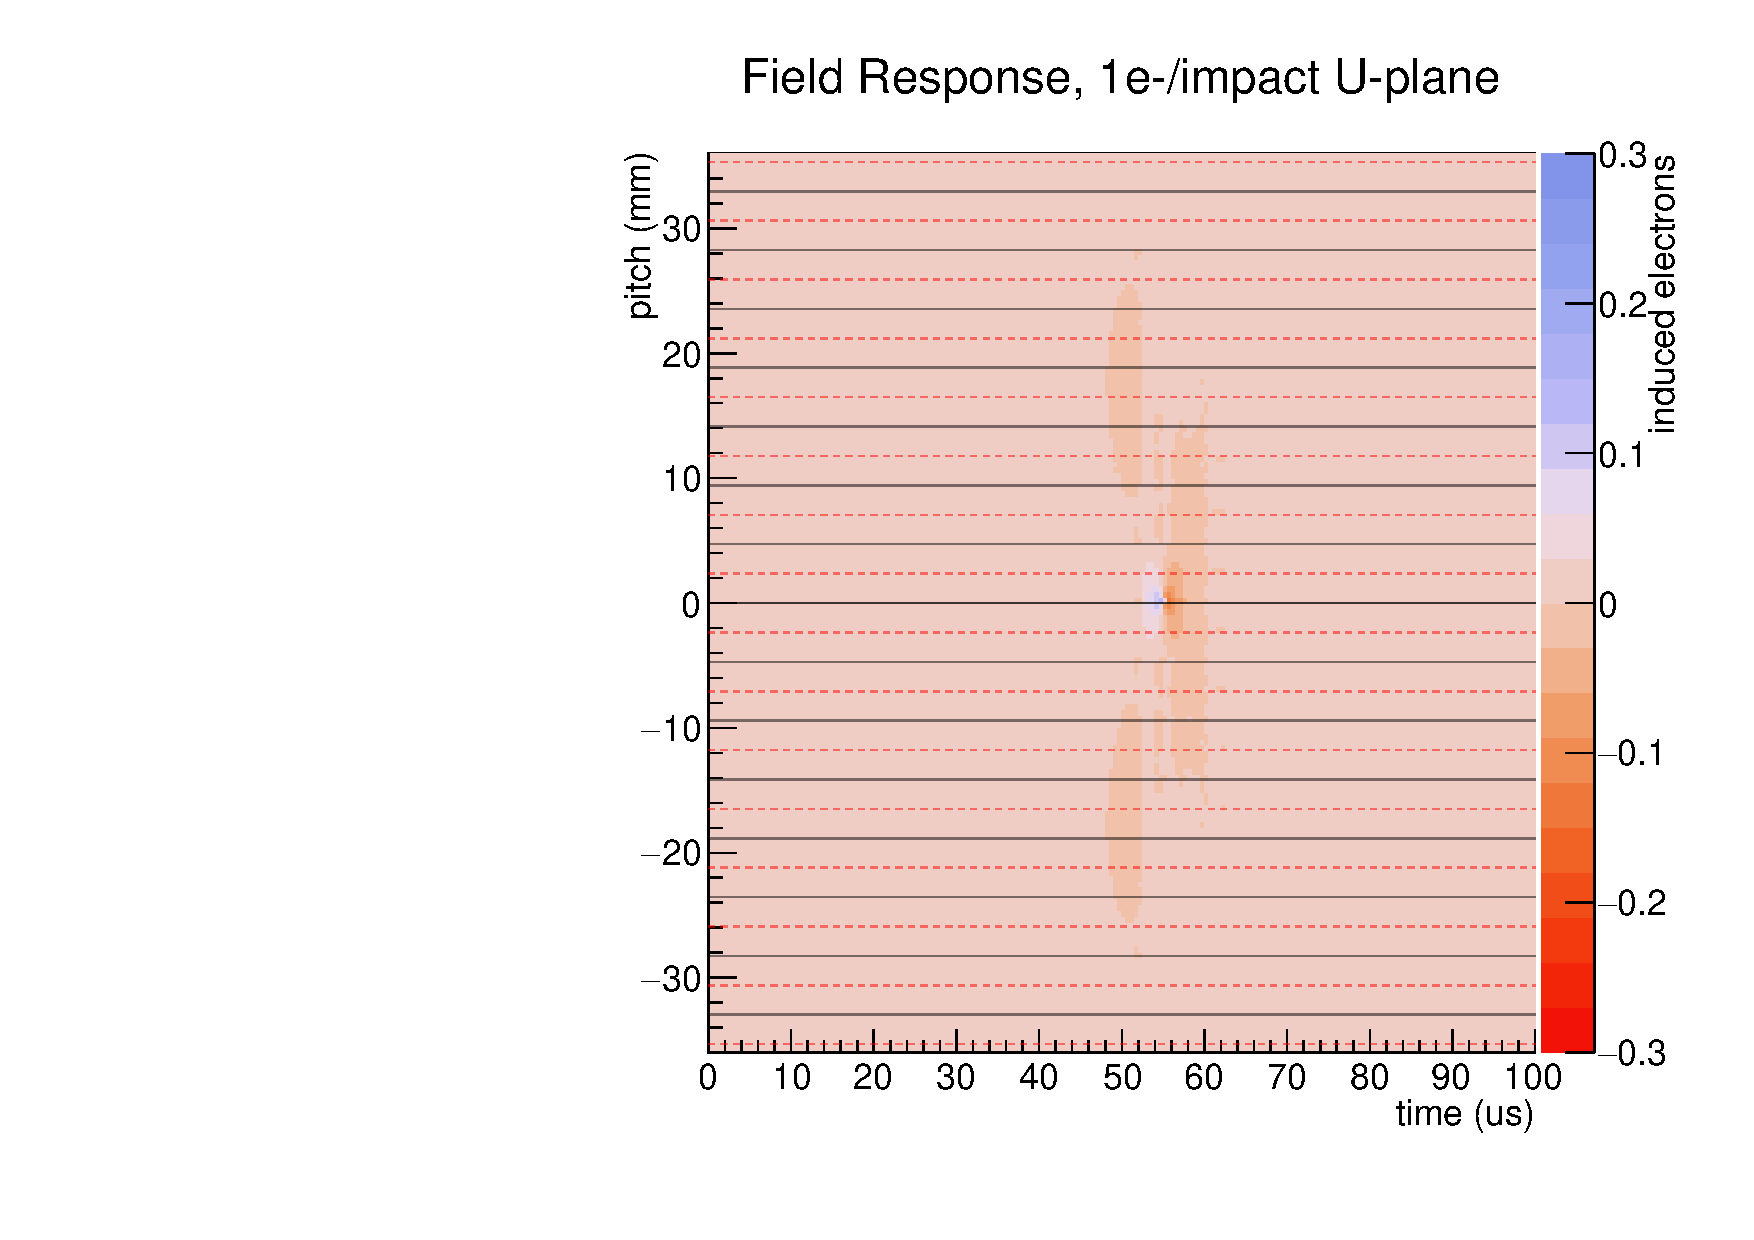
\includegraphics[width=0.3\textwidth,page=1]{test_impactresponse.pdf}
    \includegraphics[width=0.3\textwidth,page=5]{test_impactresponse.pdf}
    \includegraphics[width=0.3\textwidth,page=9]{test_impactresponse.pdf}

    \scriptsize
    Induced current of one drifting $e^{-1}$ in impact position vs. time.
  \end{center}
  
  \begin{itemize}
  \item Garfield 2D wire model, 4.71 mm pitch.
  \item $E_{field} = 500 V/cm$, $v_{drift} = $1.6 mm/$\mu$s.
  \item 21 wires, $\frac{1}{10}$pitch drift path impact positions.
  \end{itemize}
\end{frame}

\begin{frame}[fragile]
  \frametitle{Ideal Isochronous Track Response}
  
  \begin{center}
    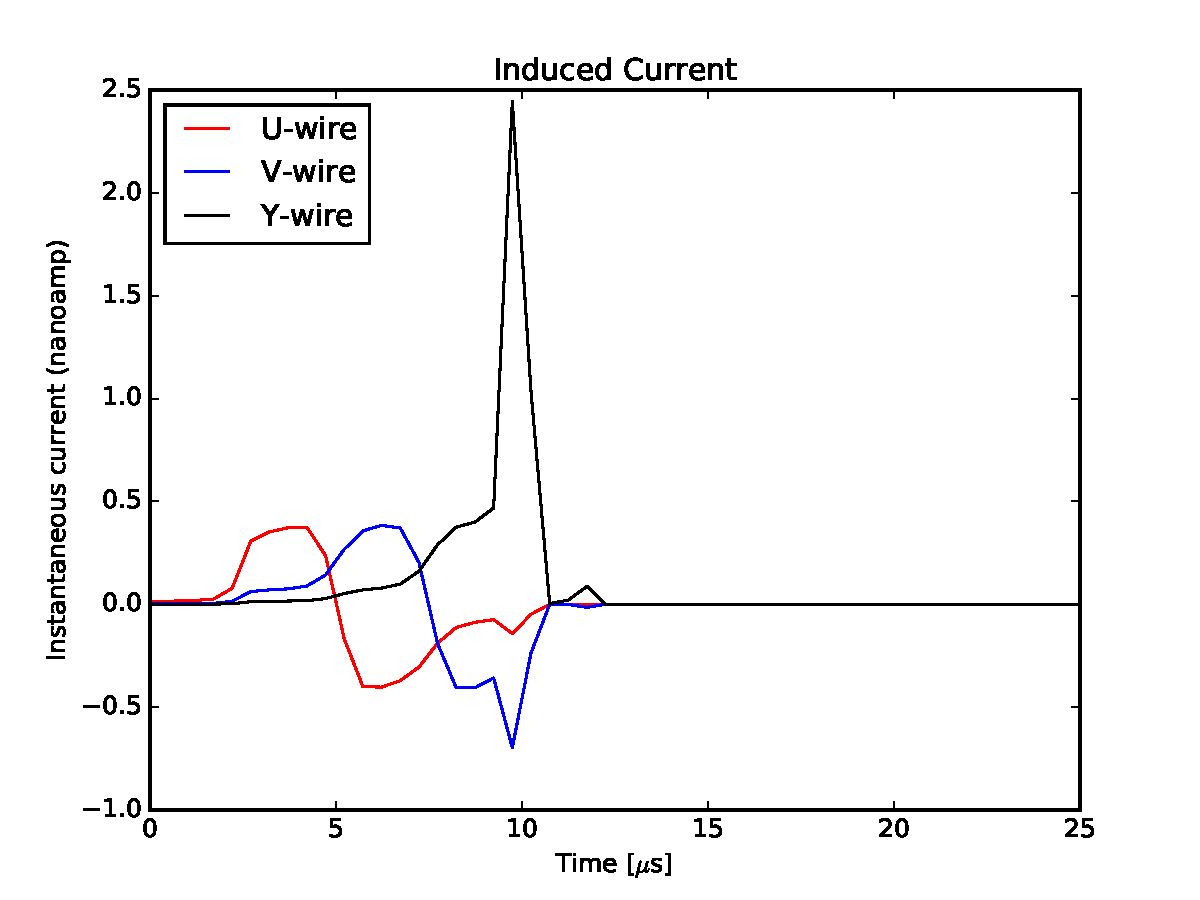
\includegraphics[width=0.3\textwidth]{dune-current.pdf}%
    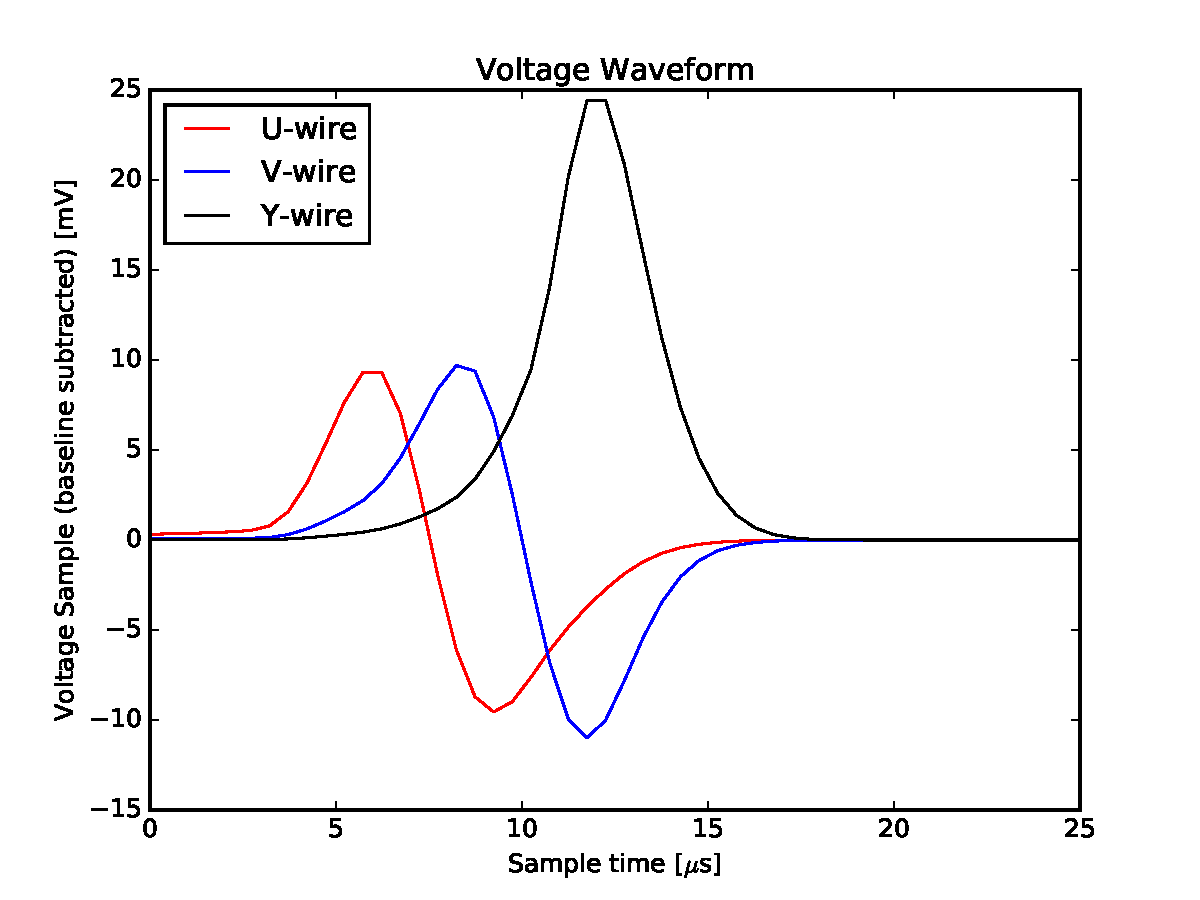
\includegraphics[width=0.3\textwidth]{dune-voltage.pdf}%
    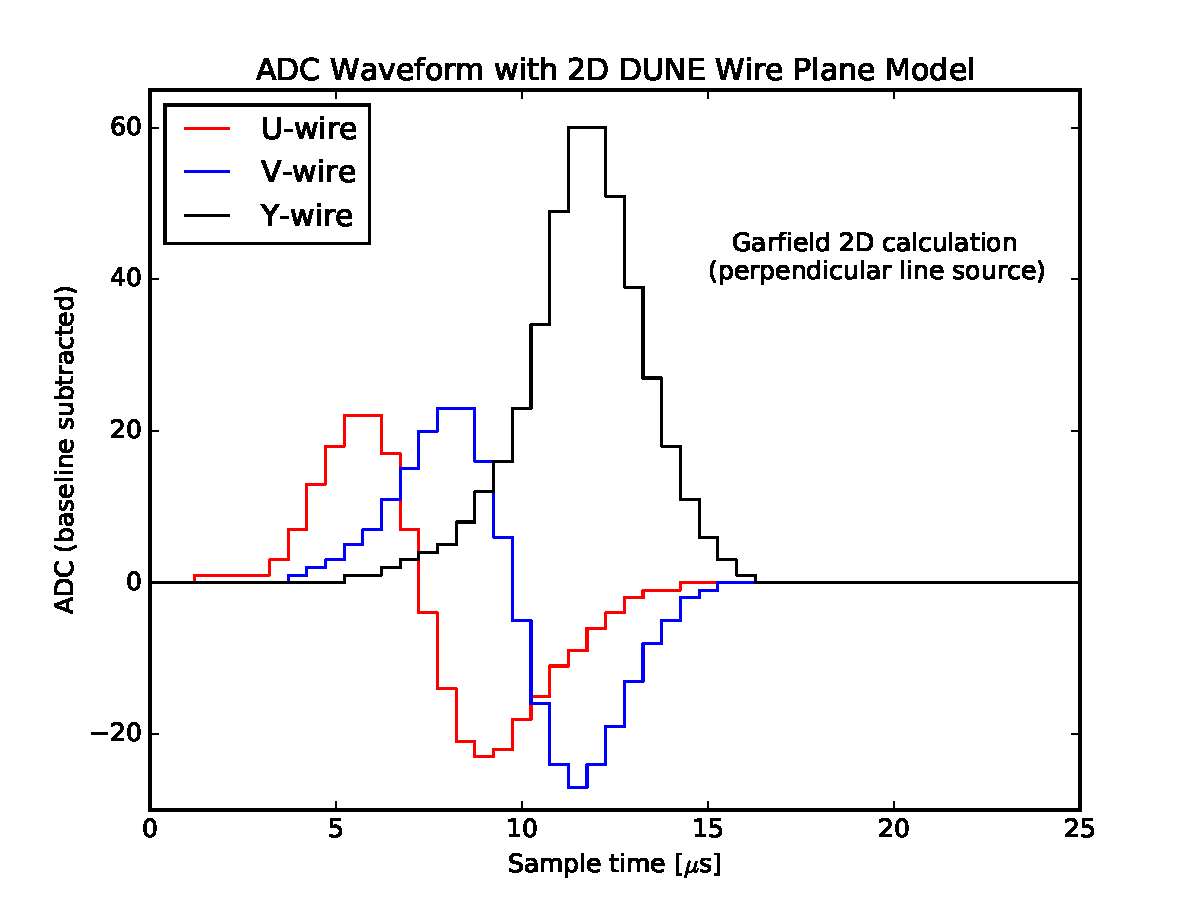
\includegraphics[width=0.3\textwidth]{dune-adc.pdf}

    \scriptsize Induced current, amplified and shaped voltage and
    digitized ADC \\
    due to ideal isochronous, MIP track (used: 16k $e^-$/pitch).
  \end{center}
  \begin{itemize}
  \item Ideal line source and $R_{field}$, $R_{elec}$ and a simple digitizer.
  \item Provides simple, understandable case that can be calculated to
    check normalization.
    \begin{itemize}\footnotesize
    \item $16,000 e^- / \si{\micro\second} = \SI{2.6}{\nano\ampere}$
    \item $16,000 e^- \times \SI{14}{\milli\volt/\femto\coulomb} = \SI{36}{\milli\volt}$
    \item $25 mV \times 1.2 \times 4096 ADC / 2V = 61V$
      \begin{itemize}\tiny
      \item[$\to$] n.b.: plots happen to use $\mu$BooNE's 1.2 post-FEE
        gain and MIP $e^-$/pitch number, but DUNE fields.  DUNE
        normalization is $\sim\frac{5}{3}\times\frac{1}{1.2} = 1.4$ higher.
      \end{itemize}
    \end{itemize}
  \end{itemize}
\end{frame}

\begin{frame}
  \frametitle{Tracked muon event}
  \begin{columns}
    \begin{column}{0.5\textwidth}
      \begin{itemize}\footnotesize
      \item LArG4 energy depositions dumped to JSON (Brooke)
      \item ADC waveforms for U/V/W planes
        \begin{itemize}\scriptsize
        \item Generated pD/SP wires and ``wire attachment number'' as channel number.
        \item Todo: full FEE channel ``shuffle''
        \end{itemize}
      \item True depo points below.
      \end{itemize}

      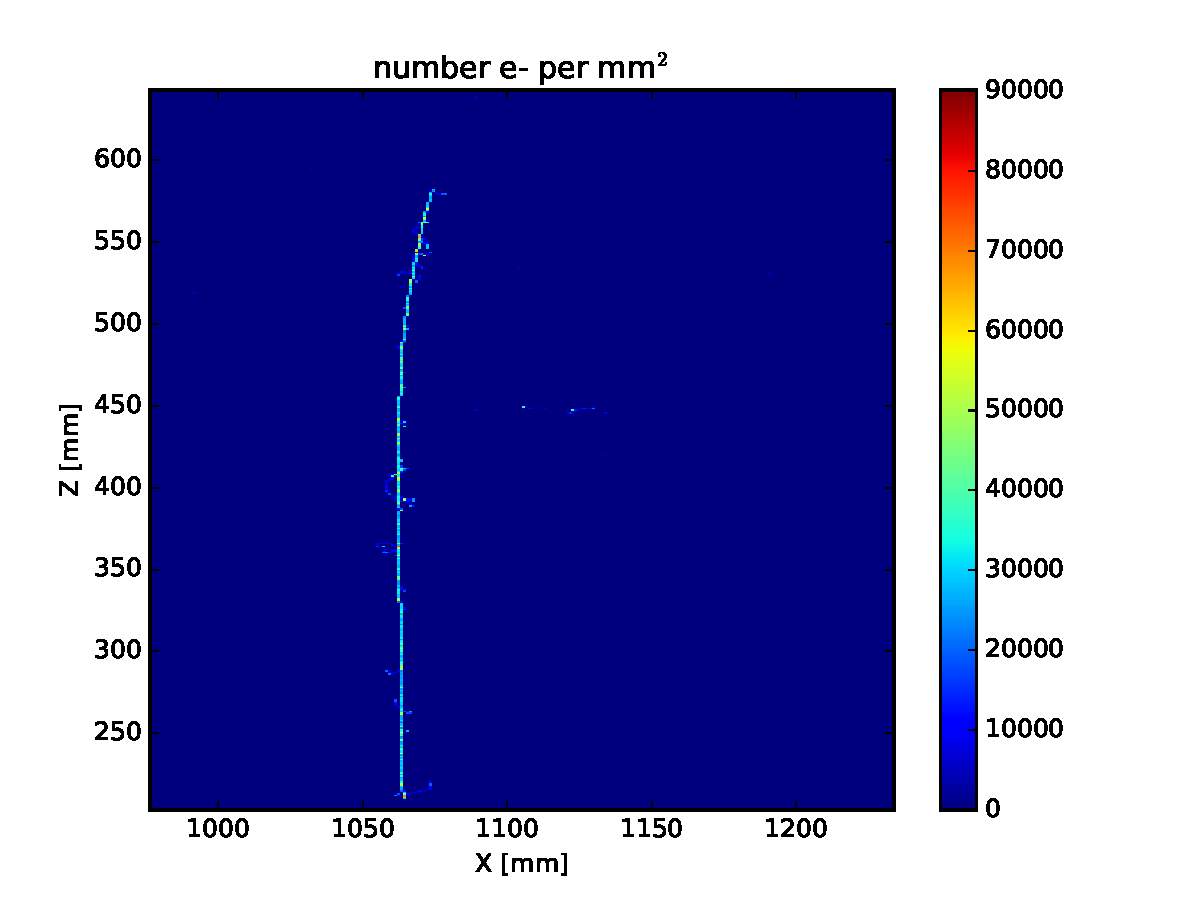
\includegraphics[width=\textwidth]{g4tuple-qsn-v1-fixed-nxz.pdf}
    \end{column}
    \begin{column}{0.5\textwidth}
      \vspace{-15mm}

      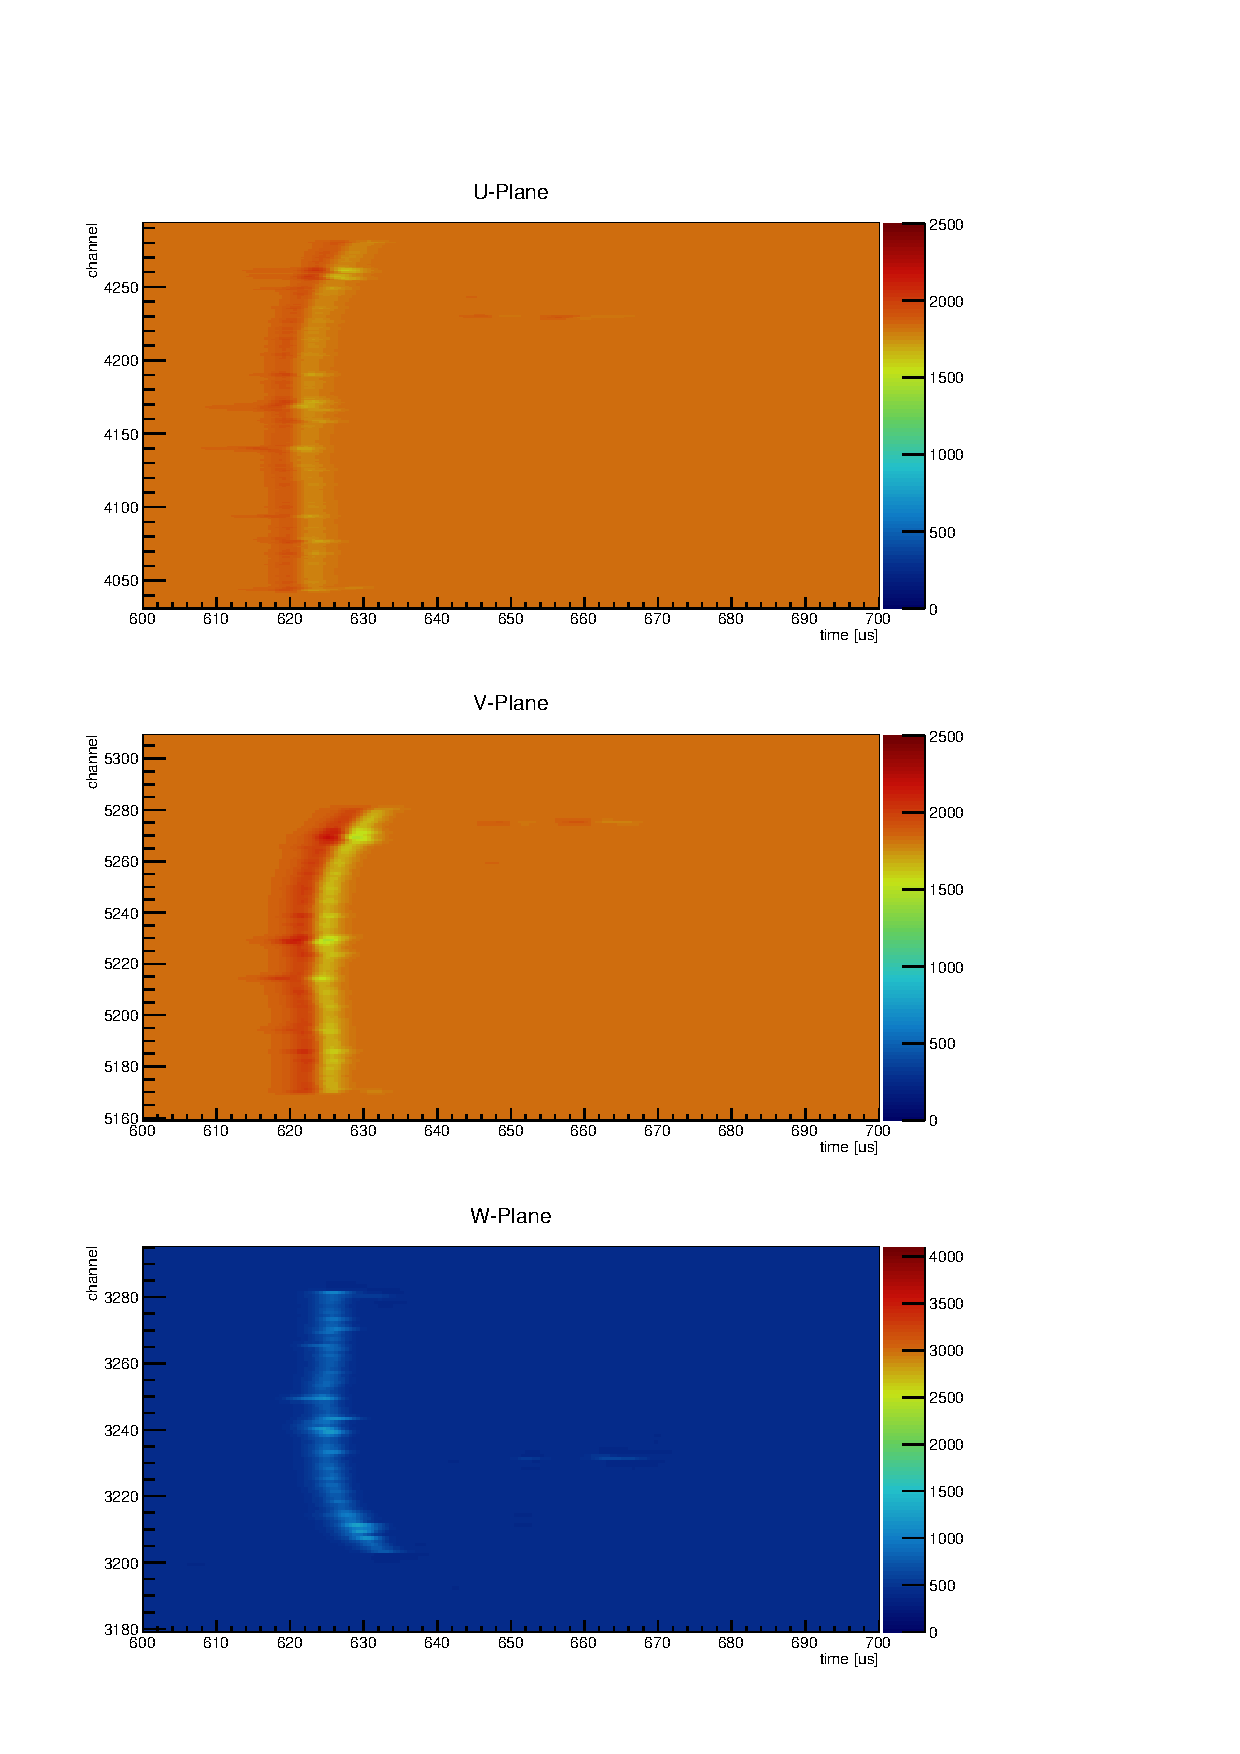
\includegraphics[width=\textwidth]{disp-pdsp-brookes-event.pdf}
    \end{column}
  \end{columns}
\end{frame}

\section{Noise Filter}

\begin{frame}
  \frametitle{Software Noise Filter}
  \begin{itemize}
  \item Class Interfaces based on per-channel and group-of-channel
    (coherent) operations.
  \item Current implementation is rather MicroBooNE-specific.
  \item Could be a basis for protoDUNE/SP noise filter but depends on
    what excess noise we actually see.
  \item \textbf{Already integrated into LArSoft} in \texttt{larwirecell} using UPS product \texttt{wirecell} (providing Wire Cell Toolkit 0.5.2 currently)
    \begin{itemize}\footnotesize
    \item Integration layer at Module level.
    \item Exposes more WCT implementation than ideal.
    \item[$\to$] Could clean this up to access WCT Compontents via Art
      Tools but this work only pays off if its reused for protoDUNE.
    \end{itemize}
  \end{itemize}
\end{frame}

\section{Signal Processing}

\begin{frame}
  \frametitle{Signal Processing}
  2D time/wire deconvolution and signal-ROI selections.
  \begin{itemize}
  \item Two filters applied in deconvolution:
    \begin{description}\footnotesize
    \item[Wiener] maximize S/N, used for signal-ROI selection.
    \item[Gaussian] preserves charge, produces final signal.
    \end{description}
  \item Signal-ROI uses ``tight'' and ``loose'' criteria and both
    local and neighboring channel info.
  \item Developed and tested on $\mu$BooNE data.
    \begin{itemize}\footnotesize
    \item Will be fully applicable to DUNE, others via configuration mods.
    \item MicroBooNE paper describing performance is in prep.
    \end{itemize}
  \item WCT sim with proper response and noise to validate SP.
  \item Initial implementation in Wire Cell \textbf{prototype} codebase.
    \begin{itemize}\footnotesize
    \item Porting to Toolkit and integration into LArSoft is high priority
    \item \textbf{Integration into LArSoft driven by paper schedule.}
      Needed sooner than for protoDUNE.
    \end{itemize}
  \end{itemize}
\end{frame}

\section{Toolkit Improvements}

\begin{frame}[fragile,fragile]
  \frametitle{Toolkit Improvements}
  \footnotesize
  \begin{itemize}
  \item Underlying configuration uses JSON.  WCT adds optional support
    for the \href{http://jsonnet.org/}{\textbf{Jsonnet} data templating language} to allow for structured configuration.
  \item Switched from Eigen3 to \textbf{FFTW3} for FFTs.  Substantial speed up
    for noise filtering, signal processing and simulation components.
  \item The \textbf{Interface} and \textbf{Dynamic Component/Plugin} based design, long existing in
    WCT, is now being applied pervasively.
  \item The nascent command line program application, \texttt{wire-cell}, is now fully usable to aggregate components into a working application. Eg, run sim:
\begin{verbatim}
$ wire-cell -c dune/fourdee.jsonnet
\end{verbatim}
  \item Input data/configuration preparation and diagnostic functions
    available as various Python CLIs, eg \textbf{generate wires} or \textbf{prepare
    Garfield responses}:
\begin{verbatim}
$ wirecell-util make-wires pdsp-wires.json.bz2
$ wirecell-sigproc convert-garfield dune_4.71.tar.gz \
    garfield-1d-3planes-21wires-6impacts-dune-v1.json.bz2
\end{verbatim}
  \end{itemize}

  
\end{frame}

\section{LArSoft Integration}

\begin{frame}
  \tableofcontents[currentsection,hideothersubsections]
\end{frame}

\begin{frame}
  \frametitle{Integration Motivations}

  WCT has substantial stand-alone functionality exposed by
  \texttt{wire-cell} CLI.  However, it is primarily a
  \textbf{toolkit} to be used in other applications

  \vfill

  WCT needs LArSoft (the framework) for some critical things:
  \begin{itemize}
  \item I/O access to official DUNE file formats. 
  \item Memory-based exchange of data products to/from
    WCT components and LS modules.
  \end{itemize}

  \vfill

  WCT lacks a subset of functionality provided by LArSoft modules:
  \begin{itemize}
  \item Particle interactions and tracking (ie, Geant4/GENIE/etc).
  \item All the many, alternative reconstruction modules.
  \end{itemize}

\end{frame}


\begin{frame}[fragile]
  \frametitle{Integration Status and Design}
  \begin{itemize}\footnotesize
  \item Wire Cell Toolkit built as \texttt{wirecell} UPS product (Lynn)
  \item LS package \texttt{larwirecell} holds layers between WCT and LS
  \item WCT heavily uses \textbf{interfaces} and
    \textbf{dynamic components}, similar to recently invented
    \textbf{Art Tool} concept.
  \item Integrate via Art Tool facade to WCT interface.
    \begin{itemize}\scriptsize
    \item[$\to$] basic model: ``\textbf{LArSoft uses Wire Cell tools}''
    \end{itemize}
  \item Same WCT app component exposed to user as CLI via
    \texttt{wire-cell} (eg, \texttt{Fourdee} sim below) will be
    exposed to LS with a single Tool facade.
  \item One Tool facade for data conversion at input/output components.
  \end{itemize}

  \begin{center}
    \includegraphics[width=\textwidth]{chain.pdf}
    
    \scriptsize
    WCT Simulation App with LS Tool facades for input/output components.
  \end{center}

\end{frame}

\section{Status and Work Needed}

\begin{frame}
  \tableofcontents[currentsection,hideothersubsections]
\end{frame}

\begin{frame}
  \frametitle{What's left to do?}

  {\scriptsize \textcolor{blue}{Areas where help is welcome are in blue}. }    

  \begin{itemize}
  \item Noise filtering
    \begin{itemize}\scriptsize
    \item Rework to better follow WCT interfaces/components patterns. (bv)
    \item \textcolor{blue}{Rework LArSoft integrating to follow Art Tool paradigm} (??, or bv)
    \end{itemize}
  \item Improved detector simulation:
    \begin{itemize}\scriptsize
    \item Long-range/fine-grained detector response, \textbf{done} (Yichen, bv).
    \item Normalization and validation, \textbf{in progress} (Hanyu, bv).
    \item Proper \textbf{noise} (Jyoti/Milind/Arbin) and \textbf{drift} (Hanyu) models: \textbf{in progress}.
      
    \item Implement FEE ``channel shuffle'' and match numbering convention. (bv)
    \item \textcolor{blue}{Integrate WCT sim components into LArSoft.} \textbf{design} (Brian, bv)
    \end{itemize}
  \item Signal processing
    \begin{itemize}\scriptsize
    \item Port prototype code into toolkit: \textbf{started} (bv, Xin)
    \item \textcolor{blue}{Validate signal processing} with simulation, develop ``truth metrics'' (Brooke), understand SP under different signal and noise assumptions.
    \item \textcolor{blue}{Integrate WCT sigproc components into LArSoft.} \textbf{design} (Brian, bv)
    \item Finish MicroBooNE paper (whole SP team)
    \end{itemize}
  \item Toolkit infrastructure miscellany
    \begin{itemize}\scriptsize
    \item Various improvements/cleanups in configuration layer and
      build/source management. (bv)
    \end{itemize}
  \end{itemize}
\end{frame}


\end{document}


%%% Local Variables:
%%% mode: latex
%%% TeX-master: t
%%% End:
